\section{Technical Foundations Established}
\label{sec:technical}

This section records the material understood so far, in our own words.
A statement of comprehension is stronger evidence of progress than a
percentage, and the argument of the full paper depends on distinctions that are
easy to state incorrectly.

\subsection{Why Shared Memory Became Unavoidable}

For roughly the first four decades of commercial computing, programs were made
faster by making one processor faster: raising the clock, and doing more work
per cycle by overlapping instruction execution.
The course's pipelining material (Sarangi \S10.4 on hazards, \S10.7 on
forwarding) and, historically, Kogge \cite{kogge1981pipelined} are precisely the
story of that overlap.
Sarangi's advanced volume continues the arc into out-of-order pipelines, where
instructions are deliberately executed in an order different from the
program's, subject only to true data and control dependences
\cite{sarangi2023nextgen}.

Two physical limits ended this.
Frequency scaling stalled because power dissipation grows steeply with clock
speed, and the returns from making a single core wider diminished.
After roughly 2005--2010 single-core performance saturated, and the transistors
Moore's law kept delivering were redirected from making one core more complex to
placing \emph{many} cores on one chip.
Hennessy and Patterson frame the same inflection as the turn to thread-level
parallelism \cite{hennessy2019quantitative}.
The multicore era was therefore not a design preference but a consequence.

Multicore hardware only delivers performance if software can use many cores at
once, and the dominant model is \textbf{shared memory}: several cores read and
write one common address space, communicating implicitly through loads and
stores rather than explicit messages (\S12.2.2).
It is attractive because it extends the uniprocessor programming model --- the
same pointers, arrays and variables.
That convenience conceals the problem this paper is about.

\subsection{The Uniprocessor Contract, and Three Ingredients of Reordering}

A programmer can reason about a sequential program only because the hardware
works hard to provide one guarantee: \textbf{the appearance of program order}.
A modern pipeline has many instructions in flight and an out-of-order core may
complete them in a scrambled sequence, but the architecture ensures the
observable result is as if instructions executed one at a time in program order.
The commit stage restores program order, and the load--store queue enforces the
necessary memory-ordering constraints.

The key point: on a uniprocessor, reordering is \emph{invisible}.
This is why a programmer of a sequential program need never learn what a store
buffer is.

Three mechanisms reorder or delay memory operations.
Each is individually benign on one core, and each becomes externally observable
through the eyes of \emph{another} core.

\begin{enumerate}[leftmargin=*,itemsep=2pt]
\item \textbf{Out-of-order execution.} A core issues independent instructions as
  operands become ready. Two loads to different addresses may execute in either
  order; a load may execute before an older store to a different address
  (\S10.11.4).
\item \textbf{Store buffers.} To avoid stalling on the latency of making a write
  globally visible, a core places it in a private FIFO queue and continues.
  Adve and Gharachorloo \cite{adve1996shared} use exactly this as their first
  example of how sequential consistency is violated.
\item \textbf{Caches and the interconnect.} Writes propagate to other cores only
  through the coherence mechanism, and different cores may learn of independent
  writes in different orders unless the system prevents it (\S11.2, \S12.4.6).
\end{enumerate}

\subsection{The Store Buffer in Detail}

The store buffer deserves particular attention, because it causes the behaviour
that defines the field.

Access to main memory costs on the order of $200$ cycles against roughly one for
arithmetic (\S11.1, \S11.3).
The store buffer works because of an asymmetry: a load produces a value
subsequent instructions need, so the core must wait; a store produces nothing
the core needs --- the value is already in hand --- so no dependence forces a
wait.
The store goes into a queue of typically 40 to 60 entries and the core proceeds.

The cost avoided is larger than it appears.
Writing to a line requires holding it in a state permitting modification; if the
core does not, it must request exclusive ownership and wait for every other
holder to relinquish its copy, potentially hundreds of cycles.

A load from the same core checks the store buffer before the cache and is served
from any matching pending entry --- \emph{store-to-load forwarding}.
This is why single-threaded programs are unaffected: a core always observes its
own writes in program order, whatever the rest of the system sees.

\begin{figure}[H]
\centering
\begin{tikzpicture}[node distance=9mm,
  unit/.style   = {draw, rounded corners=2pt, minimum width=26mm,
                   minimum height=9mm, align=center, font=\small},
  core/.style   = {unit, fill=blue!8},
  buf/.style    = {unit, fill=orange!15},
  mem/.style    = {unit, fill=black!6},
  flow/.style   = {-{Latex[length=2mm]}, thick},
  slow/.style   = {-{Latex[length=2mm]}, thick, dashed},
  lbl/.style    = {font=\scriptsize\itshape, align=center}]
  \node[core] (c)                       {Core\\\scriptsize registers, $\sim$1 cycle};
  \node[buf]  (sb) [right=22mm of c]    {Store buffer\\\scriptsize pending writes};
  \node[mem]  (l1) [below=12mm of c]    {L1 cache\\\scriptsize $\sim$4 cycles};
  \node[mem]  (mm) [below=of l1]        {Main memory\\\scriptsize $\sim$200 cycles};
  \draw[flow] (c) -- node[lbl,left]{loads} (l1);
  \draw[flow] (c) -- node[lbl,above]{stores} (sb);
  \draw[slow] (sb) |- node[lbl,pos=0.75,above]{drained later} (l1.east);
  \draw[flow] (l1) -- (mm);
  \draw[flow] (sb.north) .. controls +(0,8mm) and +(0,8mm) .. (c.north)
        node[lbl,pos=0.5,above]{forwarding};
\end{tikzpicture}
\caption{The memory path of a single core. Stores bypass the wait; the store
buffer drains asynchronously.}
\label{fig:d1-hierarchy}
\end{figure}

\noindent The essential point: \emph{the store buffer is fast precisely because
a store held in it is not yet visible to other cores}.
The invisibility is not a defect better engineering could remove.
It is the same fact as the performance benefit, seen from the other side.

\subsection{Coherence Is Not Consistency}

Before going further we must fix a distinction the course texts are careful
about and that beginners routinely blur (\S12.4.2--\S12.4.3).

\textbf{Cache coherence} concerns a \emph{single} memory location.
It guarantees that all cores agree on one total order of the writes to any one
location, and that a read eventually sees the latest write to it.
This is what MSI, MESI and MOESI provide (\S12.4.6).
It is a per-address property and says nothing about how accesses to
\emph{different} addresses are ordered.
Equivalently, coherence is \emph{per-location sequential consistency}.

\textbf{Memory consistency} concerns ordering \emph{across} locations.
If a core writes \code{x} and then writes \code{y}, can another core see the new
\code{y} but the old \code{x}?
Coherence has nothing to say, because they are different locations.

A useful way to hold the distinction: \emph{coherence makes each variable behave
sanely on its own; consistency governs how variables behave with respect to each
other.}

There is also a structural reason coherence cannot help, worth stating plainly:
\emph{the store buffer sits between the core and the cache, and therefore
upstream of the coherence protocol entirely}.
A store resting in the buffer has not been presented to the coherence
mechanism.
There is nothing for the protocol to order, invalidate or broadcast.

\begin{table}[H]
\centering
\small
\begin{tabular}{@{}p{2.5cm}p{4.9cm}p{4.9cm}@{}}
\toprule
 & \textbf{Coherence} & \textbf{Consistency} \\
\midrule
Scope        & One location & Across locations \\
Guarantee    & One total order of writes per location; eventual propagation
             & Which orderings of all memory operations are permitted \\
Mechanism    & MSI / MESI / MOESI & Store-buffer and pipeline ordering rules;
               fences \\
Acts at      & The cache & Between core and cache \\
Course ref.  & \S12.4.2, \S12.4.6 & \S12.4.3, \S12.4.7 \\
\bottomrule
\end{tabular}
\caption{Coherence versus consistency at a glance. The fourth row is why a
perfectly coherent machine still exhibits the anomaly below.}
\label{tab:d1-coh}
\end{table}

\subsection{Litmus Tests: The Vocabulary of the Field}
\label{sec:litmus}

The field's working vocabulary is a small family of tiny two- and four-thread
programs called \textbf{litmus tests}.
Each isolates one ordering question, and each memory model is characterised by
which outcomes it permits.
These recur throughout the paper and are the basis of Experiment~A.

\paragraph{Store Buffering (SB).} Initially \code{x = y = 0}.

\begin{center}
\begin{tabular}{@{}ll@{}}
\toprule
\textbf{Core 1} & \textbf{Core 2} \\
\midrule
\code{x = 1}    & \code{y = 1} \\
\code{r1 = y}   & \code{r2 = x} \\
\bottomrule
\end{tabular}
\end{center}

\noindent Can \code{r1 = 0} and \code{r2 = 0}?
Intuitively no: imagining the four operations interleaved in some single global
order, by the time both reads have happened both writes have occurred, so at
least one read should see~1.
Yet on essentially every mainstream processor, including an ordinary x86 laptop,
both reads can return zero in the same execution.
Nothing is broken.
Each core holds its write in a private store buffer and proceeds to its read
before that write has drained; both reads slip in front of both writes.

Under sequential consistency this is forbidden.
Under TSO it is permitted --- it is the \emph{defining} relaxation of TSO
\cite{sewell2010x86tso}.
This tiny program is the entire memory-consistency problem in miniature, and it
is the core of Dekker's algorithm: on hardware permitting this outcome,
Dekker's mutual exclusion admits two threads into the critical section at once.

\begin{figure}[H]
\centering
\begin{tikzpicture}[
  unit/.style = {draw, rounded corners=2pt, minimum width=30mm,
                 minimum height=10mm, align=center, font=\small},
  core/.style = {unit, fill=blue!8},
  buf/.style  = {unit, fill=orange!15},
  mem/.style  = {unit, fill=black!6, minimum width=44mm},
  flow/.style = {-{Latex[length=2mm]}, thick},
  slow/.style = {-{Latex[length=2mm]}, thick, dashed},
  lbl/.style  = {font=\scriptsize\itshape, align=center}]
  \node[core] (c0) at (0,3)    {Core 1\\\scriptsize \code{x=1; r1=y;}};
  \node[core] (c1) at (8,3)    {Core 2\\\scriptsize \code{y=1; r2=x;}};
  \node[buf]  (b0) at (0,1.4)  {Store buffer\\\scriptsize holds \code{x=1}};
  \node[buf]  (b1) at (8,1.4)  {Store buffer\\\scriptsize holds \code{y=1}};
  \node[mem]  (m)  at (4,-0.4) {Shared memory\\\scriptsize \code{x==0}, \code{y==0}};
  \draw[flow] (c0) -- (b0);
  \draw[flow] (c1) -- (b1);
  \draw[slow] (b0) -- node[lbl,left,pos=0.4]{not yet\\drained} (m.west);
  \draw[slow] (b1) -- node[lbl,right,pos=0.4]{not yet\\drained} (m.east);
  \draw[flow] (m.west) .. controls +(-3.4,0) and +(-1.6,-1.4) .. (c0.south west)
        node[lbl,pos=0.45,left]{reads 0};
  \draw[flow] (m.east) .. controls +(3.4,0) and +(1.6,-1.4) .. (c1.south east)
        node[lbl,pos=0.45,right]{reads 0};
\end{tikzpicture}
\caption{Store buffering, mechanistically. This is the operational
(abstract-machine) explanation that Sewell et al.\ make precise for x86-TSO
\cite{sewell2010x86tso}.}
\label{fig:d1-sb}
\end{figure}

\paragraph{Message Passing (MP).} Initially \code{data = 0}, \code{flag = 0}.

\begin{center}
\begin{tabular}{@{}ll@{}}
\toprule
\textbf{Core 1 (producer)} & \textbf{Core 2 (consumer)} \\
\midrule
\code{data = 42} & \code{while (flag == 0) \{\}} \\
\code{flag = 1}  & \code{r = data} \\
\bottomrule
\end{tabular}
\end{center}

\noindent When Core~2 sees \code{flag == 1}, is \code{r == 42} guaranteed?
Under SC, and for this pattern under TSO (which preserves store$\to$store
order), yes.
Under weakly ordered models --- ARM, POWER, Alpha --- \textbf{not without a
barrier}: the producer's two writes can become visible out of order, or the
consumer's two reads can be reordered, so the consumer sees the flag set and
reads stale data.
This is the single most important pattern in real concurrent code and the reason
acquire/release fences exist \cite{maranget2012tutorial}.

\paragraph{Load Buffering (LB).} Initially \code{x = y = 0}.
Core~1 reads \code{x} then writes \code{y}; Core~2 reads \code{y} then writes
\code{x}.
Can both reads return 1?
This requires each core's read to be reordered after its write.
Forbidden by SC and TSO; allowed by some weak models.
It distinguishes models that preserve load$\to$store order from those that do
not.

\paragraph{Independent Reads of Independent Writes (IRIW).}
Two cores write; two others read both variables in opposite orders.
Can the two observers disagree about the order in which the two independent
writes occurred?
Models permitting this are \textbf{not multicopy atomic} --- a write can become
visible to some cores before others.
Classic POWER and ARMv7 permit it; x86-TSO does not, and ARMv8 was revised in
2018 to forbid it.
This is the cleanest probe of write atomicity, one of the deepest axes in the
subject \cite{alglave2014herding}.

\begin{table}[H]
\centering
\small
\begin{tabular}{@{}lccccc@{}}
\toprule
\textbf{Test} & \textbf{SC} & \textbf{x86-TSO} & \textbf{SPARC PSO} &
\textbf{ARMv7 / POWER} & \textbf{ARMv8} \\
\midrule
SB   & Forbidden & Allowed   & Allowed   & Allowed & Allowed \\
MP   & Forbidden & Forbidden & Allowed   & Allowed & Allowed \\
LB   & Forbidden & Forbidden & Forbidden & Allowed & Allowed \\
IRIW & Forbidden & Forbidden & Forbidden & Allowed & Forbidden \\
\bottomrule
\end{tabular}
\caption{Canonical litmus tests and whether each model permits the surprising
outcome. To be confirmed empirically in Experiment~A and cross-checked against
\code{herd7} predictions.}
\label{tab:d1-litmus}
\end{table}

\subsection{The Design Space of Hardware Models}

A \textbf{memory consistency model} is the architecturally visible specification
of which orderings a multiprocessor may exhibit, and therefore which values a
read may return.
It is a contract: hardware promises no less, software may assume no more.

Models are characterised by which of four program-order pairs they preserve, and
by whether they are multicopy atomic.

\begin{table}[H]
\centering
\small
\begin{tabular}{@{}lcccccl@{}}
\toprule
\textbf{Model} & \textbf{S$\to$L} & \textbf{S$\to$S} & \textbf{L$\to$L} &
\textbf{L$\to$S} & \textbf{MCA} & \textbf{Deployed in} \\
\midrule
Sequential consistency & \checkmark & \checkmark & \checkmark & \checkmark & \checkmark & --- \\
TSO       & $\times$ & \checkmark & \checkmark & \checkmark & \checkmark & x86, SPARC \\
PSO       & $\times$ & $\times$   & \checkmark & \checkmark & \checkmark & SPARC \\
Weak / RMO& $\times$ & $\times$   & $\times$   & $\times$   & varies & ARM, POWER, RISC-V \\
Release consistency & $\times$ & $\times$ & $\times$ & $\times$ & varies & C++11, ARMv8 \\
\bottomrule
\end{tabular}
\caption{Program-order pairs preserved by each model; MCA denotes multicopy
atomicity. Every commercially deployed instruction set sits strictly below
sequential consistency.}
\label{tab:d1-models}
\end{table}

\noindent The tension is visible in the table.
At the top, intuition is sound and the programmer needs no special knowledge ---
but naively the core must stall on every store, abandoning the store buffer and
much of its performance.
At the bottom the hardware runs at full speed and the programmer is handed
fences.
Empirically, programmers place them wrongly; the resulting defects are
probabilistic, appear only under particular thread placements, and typically
vanish under a debugger.

\subsection{Historical Development}

The industry did not arrive at weak models by oversight.
It argued for them, under assumptions that have since changed.

\begin{figure}[H]
\centering
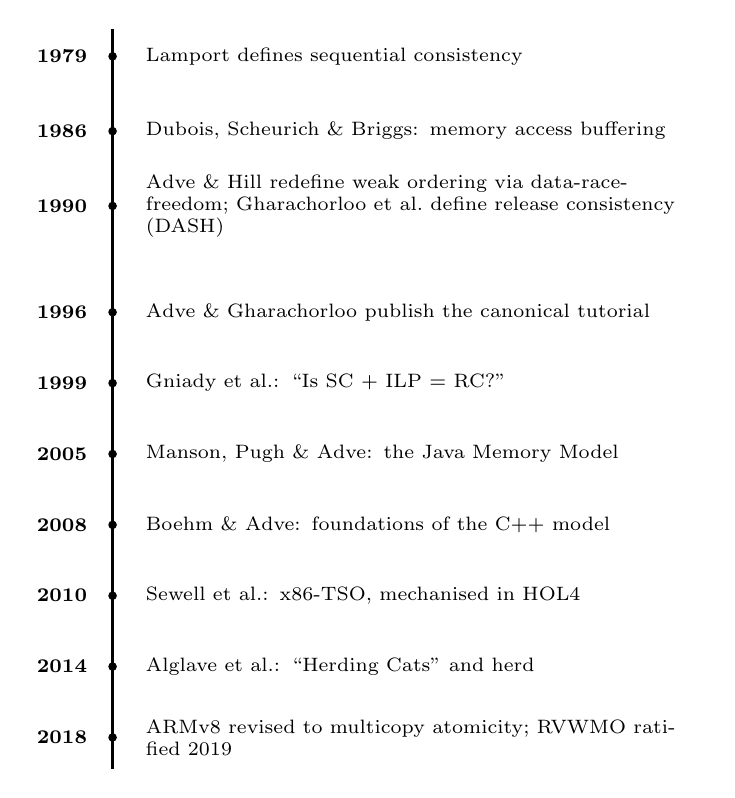
\begin{tikzpicture}[
    yr/.style={font=\scriptsize\bfseries},
    ev/.style={font=\scriptsize, align=left, anchor=west, text width=70mm},
    dot/.style={circle, fill=black, inner sep=1.1pt}]
  \draw[thick] (0,0) -- (0,-9.4);
  \foreach \y/\year/\text in {%
    -0.35/1979/{Lamport defines sequential consistency},
    -1.3/1986/{Dubois, Scheurich \& Briggs: memory access buffering},
    -2.25/1990/{Adve \& Hill redefine weak ordering via data-race-freedom;
                Gharachorloo et al.\ define release consistency (DASH)},
    -3.6/1996/{Adve \& Gharachorloo publish the canonical tutorial},
    -4.5/1999/{Gniady et al.: ``Is SC + ILP = RC?''},
    -5.4/2005/{Manson, Pugh \& Adve: the Java Memory Model},
    -6.3/2008/{Boehm \& Adve: foundations of the C++ model},
    -7.2/2010/{Sewell et al.: x86-TSO, mechanised in HOL4},
    -8.1/2014/{Alglave et al.: ``Herding Cats'' and \code{herd}},
    -9.0/2018/{ARMv8 revised to multicopy atomicity; RVWMO ratified 2019}}
  {
    \node[dot] at (0,\y) {};
    \node[yr, anchor=east] at (-0.2,\y) {\year};
    \node[ev] at (0.3,\y) {\text};
  }
\end{tikzpicture}
\caption{Chronology of memory consistency models.}
\label{fig:d1-timeline}
\end{figure}

\paragraph{1979 --- the definition.}
Lamport's paper \cite{lamport1979multiprocessor} is two pages and does not argue
that sequential consistency is desirable; it assumes so, and asks what a
hardware implementation must satisfy.
Its significance is that it made the assumption explicit and therefore
falsifiable: once SC had a definition, one could build a machine that
demonstrably violated it and argue that doing so was a good idea.

\paragraph{1986--1990 --- the case for relaxation.}
Dubois, Scheurich and Briggs \cite{dubois1986memory} observed that SC binds at
every memory operation, whereas programs need ordering only where threads
communicate.
Adve and Hill \cite{adve1990weak} then inverted the framing: rather than
defining weak ordering as a hardware behaviour, they defined it as a contract
--- write a data-race-free program and the hardware will appear sequentially
consistent.
This is the most consequential idea in the field.
Gharachorloo et al.\ \cite{gharachorloo1990memory} refined it with release
consistency, noting acquire and release each constrain only one direction and so
admit cheaper implementations.

\paragraph{The cost of the settlement.}
The bargain rested on a premise that received less scrutiny than it deserved:
that programmers would write data-race-free programs.
Java shipped in 1995 with a model that proved simultaneously too weak for the
idioms programmers used and too strong for standard compiler optimisations; it
was replaced wholesale by JSR-133 \cite{manson2005java}.
C++ had no memory model at all until C++11 \cite{boehm2008foundations}.
Alglave et al.\ \cite{alglave2014herding} formalised the published ARM and POWER
manuals and found they did not describe the machines --- permitting executions
no chip produced and forbidding some that chips did.
ARM's 2018 revision to multicopy atomicity was a \emph{strengthening} of a
shipped architecture, undertaken because the weaker model was too hard to reason
about.

\paragraph{2010 onwards --- rigour.}
Sewell et al.\ \cite{sewell2010x86tso} gave x86-TSO in both operational and
axiomatic form and proved the two equivalent in HOL4.
Alglave et al.\ \cite{alglave2014herding} unified the axiomatic treatment and
supplied executable models.
The field is now unusually rigorous for computer architecture, and this rigour
is what makes the experimental programme of this paper possible.

\subsection{Why This Matters: Three Stakes}

The problem is not academic.
Adve and Gharachorloo \cite{adve1996shared} frame the canonical trio:

\begin{description}[leftmargin=1.9cm,style=nextline,font=\normalfont\bfseries]
\item[Correctness] Synchronisation code --- locks, lock-free structures, the
  internals of language runtimes and OS kernels --- is correct only relative to
  a memory model. The same C code can be correct on x86 and subtly broken on
  ARM. Sewell et al.\ \cite{sewell2010x86tso} verify a Linux spinlock against
  x86-TSO, and the proof depends on TSO's specific guarantees.
\item[Portability] Because models differ, a program reasoned about on one
  architecture may misbehave on another. This is what pushed the problem
  \emph{up} into programming languages.
\item[Performance] Every ordering guarantee has a cost. Enforcing sequential
  consistency naively means a core often cannot proceed past a memory operation
  until it is globally visible, discarding the very buffering that makes cores
  fast. Quantifying this trade-off is Experiment~B.
\end{description}

\subsection{Language-Level Memory Models}

Hardware models are not the whole story.
Application programmers write in C, C++, Java, Rust and Go, and the compiler is
\emph{itself} a source of reordering --- it hoists, sinks and eliminates memory
accesses.
A correct concurrent program therefore needs a contract with the \emph{language},
not just the hardware.

\paragraph{SC-DRF: the unifying idea.}
The most important idea in language memory models is \textbf{SC for
data-race-free programs}, whose lineage runs from Adve and Hill
\cite{adve1990weak} through the Java and C++ models.
\emph{If a program has no data races --- every pair of conflicting accesses is
ordered by synchronisation --- the programmer is guaranteed sequential
consistency, even though hardware and compiler are relaxed.}
The bargain: programmers promise to synchronise properly; in return the system
promises intuitive semantics.
Relaxation is confined to ordinary accesses in correctly synchronised code,
where it is invisible, and to explicitly tagged atomics, where the programmer
opts into weaker guarantees knowingly.

\paragraph{Java (2005).}
Java is memory-safe and sandboxed, so it cannot allow racy programs to do
\emph{anything} --- undefined behaviour would break the security model.
The Java Memory Model \cite{manson2005java} therefore had the hard job of giving
SC-DRF \emph{and} bounding the behaviour of racy programs, via happens-before
and causality constraints forbidding values appearing ``out of thin air''.
It is the first industrial-strength language memory model, and the fact that
several proposed versions had subtle flaws is itself a lesson in how non-obvious
this territory is.

\paragraph{C++11 and \code{std::atomic}.}
C++ prioritises performance and control, and exposes the trade-off directly
through \code{std::atomic} operations parameterised by a \code{memory\_order}
\cite{boehm2008foundations}:

\begin{itemize}[leftmargin=*,itemsep=1pt]
\item \code{memory\_order\_seq\_cst} --- the default; participates in a single
  total order of all seq\_cst operations. Strongest and most expensive.
\item \code{memory\_order\_acquire} / \code{memory\_order\_release} --- the
  acquire/release pair from release consistency, giving exactly the ordering MP
  needs without a full fence.
\item \code{memory\_order\_acq\_rel} --- both, for read-modify-write operations.
\item \code{memory\_order\_relaxed} --- atomicity only, no ordering. Cheapest;
  used for counters and flags where ordering is not required.
\end{itemize}

This is the cleanest place to \emph{measure} the trade-off empirically, because
the same program can be recompiled with different tags and its performance
observed.
That is precisely the design of Experiment~B.

\paragraph{The compiler as a reordering agent.}
Even on a strongly ordered CPU like x86, a program can exhibit weak-memory bugs
because the \emph{compiler} reordered accesses at \code{-O2}.
The language memory model is what makes compiler optimisations legal only up to
the point where they remain invisible to correctly synchronised code.
Vafeiadis et al.\ \cite{vafeiadis2015common} showed that some ``obvious''
optimisations are unsound under the C11 model --- evidence that the language
layer is as subtle as the hardware layer, and the reason Experiment~B measures
\emph{compiled} behaviour rather than reasoning about source.

\subsection{Specifying and Verifying Memory Models}

Where the preceding subsections show breadth, this one shows depth: how much
rigour a single point in the space demands.
This is where an introductory course treatment hands off to the research
literature.

\paragraph{Two specification styles.}
Models are given \emph{operationally} --- define an idealised machine (cores,
store buffers, drain rules) and declare an execution legal iff that machine can
produce it --- or \emph{axiomatically} --- define relations over operations
(program order, reads-from, coherence) and declare an execution legal iff those
relations satisfy stated acyclicity axioms.
The operational form is intuitive and close to hardware; the axiomatic form is
compact, comparable across models, and tool-friendly.

A central technical activity is \emph{proving the two coincide} for a given
architecture --- that the x86-TSO store-buffer machine accepts exactly the
executions the x86-TSO axioms allow.
Sewell et al.\ did this in the HOL4 proof assistant \cite{sewell2010x86tso}.
It matters because the operational form guides implementers and the axiomatic
form guides tool-builders; a proof that they agree means both communities are
discussing the same model.

\paragraph{Litmus testing and \code{herdtools7}.}
The empirical backbone of the field is litmus testing: take a small program with
a known interesting outcome, run it billions of times on real hardware to see
whether the outcome occurs, and compare against what a candidate model predicts.
The \code{herdtools7} suite operationalises this --- \code{litmus7} runs tests on
hardware, \code{herd7} simulates a model --- and is the direct descendant of the
``herding cats'' methodology \cite{alglave2014herding}.
This is the tooling Experiment~A will use.

\paragraph{The \code{.cat} language.}
A significant modern development is that axiomatic models are written in a small
domain-specific language, \code{.cat}, as sets of relation definitions and
acyclicity constraints, and then \emph{executed} by \code{herd7}.
A memory model becomes a short, precise, runnable file; the x86-TSO, ARMv8,
POWER, RISC-V and C++11 models all exist as \code{.cat} files.
This closes the loop between specification and testing and is why the field is
unusually rigorous for computer architecture.

\paragraph{Verification.}
Beyond testing there is proof: that a microarchitecture or compiler respects a
model.
This includes microarchitectural consistency verification, compiler-correctness
results for the mapping from C++11 atomics to ARM and POWER barriers, and
ongoing work on RVWMO and GPU models.
A recent survey \cite{weakmemory2025survey} collects the current state.

\subsection{Annotated Literature Survey}

The sources below are grouped by role.
Annotations state why each matters and where the paper uses it.

\paragraph{Foundational definitions.}
Lamport \cite{lamport1979multiprocessor} defines sequential consistency in two
pages; the origin point, and our reference model.
Adve and Gharachorloo \cite{adve1996shared} give the best synthesis of the
relaxed-model zoo, organised by the program-order-relaxation and write-atomicity
axes; the backbone of our design-space treatment.

\paragraph{Relaxed-model origins.}
Dubois, Scheurich and Briggs \cite{dubois1986memory} introduced formal
relaxation via access buffering and the idea of ordering only at synchronisation.
Adve and Hill \cite{adve1990weak} supplied the programmer-centric reframing
(SC-for-DRF) that underlies every later language model.
Gharachorloo et al.\ \cite{gharachorloo1990memory} introduced release
consistency and the acquire/release distinction, realised in Stanford DASH and
reused verbatim by C++11.

\paragraph{Language-level models.}
Manson, Pugh and Adve \cite{manson2005java} on the Java Memory Model; Boehm and
Adve \cite{boehm2008foundations} on the foundations of C++11 atomics; Vafeiadis
et al.\ \cite{vafeiadis2015common} showing the compiler layer is as subtle as
the hardware.

\paragraph{Rigorous hardware models and tooling.}
Sewell et al.\ \cite{sewell2010x86tso} give x86-TSO in operational and axiomatic
form, proved equivalent in HOL4 and demonstrated on a real spinlock --- our
reference model for the hardware experiments.
Maranget, Sarkar and Sewell \cite{maranget2012tutorial} provide the accessible
entry to ARM and POWER.
Alglave, Maranget and Tautschnig \cite{alglave2014herding} give the unified
axiomatic framework, the \code{herd} simulator and the data-mining methodology
that became \code{herdtools7} --- our core experimental tooling.

\paragraph{Reference texts.}
Nagarajan et al.\ \cite{nagarajan2020primer} is the standard modern textbook,
open access, with chapters on GPU models and formal tools.
Course anchors are Sarangi \cite{sarangi2025basic,sarangi2023nextgen}, with
Hennessy and Patterson \cite{hennessy2019quantitative} and Kogge
\cite{kogge1981pipelined} for the pipelining roots.

\subsection{Open Problems}

The subject spans four layers --- hardware models, language models,
specification styles, and verification --- and a term paper can travel a long
way horizontally, but the payoff is in choosing a vertical slice and going deep.
Problems the paper can point to, or engage with:

\begin{enumerate}[leftmargin=*,itemsep=2pt]
\item \textbf{Out-of-thin-air values.} Language models still struggle to forbid
  absurd self-justifying outcomes in relaxed code without also forbidding
  legitimate compiler optimisations.
\item \textbf{Heterogeneous and scoped consistency.} CPU--GPU systems with
  scoped synchronisation lack a single clean model.
\item \textbf{Persistent memory ordering.} Non-volatile memory adds a
  \emph{durability} order on top of the visibility order.
\item \textbf{RVWMO adoption and verification.} A young, open, formally specified
  model whose hardware conformance is still maturing.
\item \textbf{Was the rejection of sequential consistency correct?} SC was
  rejected on performance grounds around 1990, on machines that did not
  speculate. Gniady et al.\ \cite{gniady1999sc} argued that a speculative core
  --- which already has coherence invalidations for detection and a squash path
  for recovery --- can enforce SC cheaply, and later work extended this
  \cite{ceze2007bulksc,blundell2009invisifence,marino2011sc}. No shipping
  processor implements SC, and the gap is unexplained.
\end{enumerate}

\paragraph{Where our slice sits.}
The paper's chosen depth is the x86-TSO corner: strong enough to reason about
cleanly, rigorously specified, well tooled, and directly connected to the C++11
model the microbenchmarks target.
This lets the work be concrete and reproducible while still touching the
frontier through the survey.
